\documentclass[handout]{beamer}


\usetheme{default}
\usepackage{subfigure}
\usepackage{amsmath}
\usepackage{Sweave}
\usepackage{graphicx}
\usepackage{color}
\usepackage{multicol}
\usepackage{bm}


\author{Patrick Lam}
\title{Summarizing the Posterior}
\date{}
%\date{September 29, 2008}

\begin{document}

\newcommand{\red}{\textcolor{red}}
\newcommand{\blue}{\textcolor{blue}}
\newcommand{\purple}{\textcolor{purple}}

\frame{\titlepage}

\begin{frame}
\frametitle{Outline}
\tableofcontents
\end{frame}

\section{Marginal Distributions and Integration}

\begin{frame}
\frametitle{Outline}
\tableofcontents[currentsection]
\end{frame}

\begin{frame}
\frametitle{Marginal Distributions}
\pause
Suppose you have a joint distribution of two parameters, $p(\theta_1, \theta_2)$.\\
\pause
\bigskip
How do you get the marginal distribution of $p(\theta_1)$?  \pause \red{Integrate}
\pause
\begin{eqnarray*}
p(\theta_1) = \int p(\theta_1, \theta_2) d\theta_2
\end{eqnarray*}
\pause
This works for more than two parameters as well:
\pause
\begin{eqnarray*}
p(\theta_1) = \int \int p(\theta_1, \theta_2, \theta_3) d\theta_2 d\theta_3
\end{eqnarray*}
\pause
We can sometimes do the integrals analytically, but more often than
not we want to simulate from the marginal distribution.
\end{frame}

\begin{frame}
\frametitle{Integrating a Grid}
\pause
Suppose we were doing a grid approximation of a bivariate distribution
of $\theta_1$ and $\theta_2$. \\
\begin{multicols}{2}
\pause
\scriptsize
\begin{table}[!htp]
\begin{center}
\caption{Joint Grid}
\begin{tabular}{|c|c|c|}
\hline
$\theta_1$ & $\theta_2$ & $p(\theta_1, \theta_2)$\\
\hline
0 & 0 & 0.4 \\
0 & 0.5 & 0.7\\
0 & 1 & 0.5\\
0.5 & 0 & 0.6\\
0.5 & 0.5 & 0.8\\
0.5 & 1 & 0.8\\
1 & 0 & 0.7\\
1 & 0.5 & 0.6\\
1 & 1 & 0.5\\
\hline
\end{tabular}
\end{center}
\end{table}
\pause
\begin{eqnarray*}
p(\theta_1 = 0) &=& 0.4 + 0.7 + 0.5 = 1.6\\
p(\theta_1 = 0.5) &=& 0.6+0.8+0.8 = 2.2\\
p(\theta_1 = 1) &=& 0.7+0.6+0.5 = 1.8
\end{eqnarray*}
\pause
\begin{table}[!htp]
\begin{center}
\caption{Marginal Grid}
\begin{tabular}{|c|c|}
\hline
$\theta_1$  & $p(\theta_1)$\\
\hline
0 & 1.6\\
0.5 & 2.2\\
1 & 1.8\\
\hline
\end{tabular}
\end{center}
\end{table}
\end{multicols}
\pause
\normalsize
We can sample from the marginal grid to get simulations from the
marginal distribution $p(\theta_1)$. 
\end{frame}

\begin{frame}
\frametitle{Integrating Simulations}
\pause
Now suppose that we have a bunch of simulated draws from the joint
distribution (obtained either by sampling from the joint grid or other
simulation methods).

\begin{multicols}{2}
\scriptsize
\begin{table}[!htp]
\begin{center}
\caption{Joint Simulations}
\begin{tabular}{|c|c|c|}
\hline
Draw $\#$  & $\theta_1$ & $\theta_2$\\
\hline
1 & 0.5 & 1\\
2 & 1 & 0\\
3 & 1 & 0\\
4 & 0 & 1\\
5 & 0 & 0.5\\
6 & 0.5 & 0.5\\
7 & 1 & 0.5\\
8 & 0.5 & 0\\
9 & 0.5 & 1\\
10 & 0.5 & 0.5\\
\hline
\end{tabular}
\end{center}
\end{table}

\pause
\begin{table}[!htp]
\begin{center}
\caption{Marginal Simulations}
\begin{tabular}{|c|c|}
\hline
Draw $\#$  & $\theta_1$ \\
\hline
1 & 0.5 \\
2 & 1 \\
3 & 1 \\
4 & 0 \\
5 & 0 \\
6 & 0.5 \\
7 & 1 \\
8 & 0.5 \\
9 & 0.5 \\
10 & 0.5 \\
\hline
\end{tabular}
\end{center}
\end{table}
\end{multicols}
\pause
To obtain simulations from the marginal distribution, we simply drop
the simulated values from the other parameter(s).
\end{frame}

\section{Summarizing the Posterior}

\begin{frame}
\frametitle{Outline}
\tableofcontents[currentsection]
\end{frame}

\begin{frame}
\frametitle{Summarizing the Posterior}
\pause
Suppose we now have either analytical or simulated \textcolor{blue}{posterior}.  \\
\pause
\bigskip
What are some of the ways we can summarize the \textcolor{blue}{posterior}? \\
\pause
\bigskip
Consider the previous example of the beta-binomial model with a
\textcolor{red}{Beta(1,1) prior} (uniform) and a
\textcolor{blue}{Beta($y+\alpha, n-y+\beta$) posterior}, where $n=500$,
$y = 285$, $\alpha = 1$, and $\beta = 1$.
\end{frame}

\begin{frame}[fragile]
\frametitle{Posterior Mean}
\pause
Analytically:
\begin{eqnarray*}
\frac{y+\alpha}{(y+\alpha) + (n-y+\beta)} = \frac{286}{286+216}
\approx 0.57\\
\end{eqnarray*}
\pause
\bigskip
Simulation:
\tiny
\begin{Schunk}
\begin{Sinput}
> a <- 1
> b <- 1
> posterior.unif.prior <- rbeta(10000, shape1 = 285 + a, shape2 = 500 - 
+     285 + b)
> mean(posterior.unif.prior)
\end{Sinput}
\begin{Soutput}
[1] 0.5699
\end{Soutput}
\end{Schunk}
\normalsize
\end{frame}

\begin{frame}[fragile]
\frametitle{Posterior Variance}
\pause
Analytically:
\begin{eqnarray*}
\frac{(y+\alpha)(n-y+\beta)}{[(y+\alpha) + (n-y+\beta)]^2 [(y+\alpha)
+ (n-y+\beta) + 1]} % = \\ \frac{(286)(216)}{(286+216)^2 (286+216+1)}
\approx  0.00049\\
\end{eqnarray*}
\pause
\bigskip
Simulation:
\tiny
\begin{Schunk}
\begin{Sinput}
> var(posterior.unif.prior)
\end{Sinput}
\begin{Soutput}
[1] 0.0004832
\end{Soutput}
\end{Schunk}
\normalsize
\pause
Take the square root for standard deviation.
\end{frame}

\begin{frame}[fragile]
\frametitle{Posterior Probability $0.5 < \pi < 0.6$}
\pause
Analytically:
\begin{eqnarray*}
\int_{0.5}^{0.6}  \frac{\Gamma ((y+\alpha) + (n-y+\beta))}{\Gamma (y+\alpha)
\Gamma (n-y+\beta)} \pi^{(y+\alpha - 1)} (1 - \pi)^{(n-y+\beta-1)}
d\pi \approx 0.91\\
\end{eqnarray*}
\pause
\bigskip
Simulation:
\tiny
\begin{Schunk}
\begin{Sinput}
> mean(posterior.unif.prior > 0.5 & posterior.unif.prior < 0.6)
\end{Sinput}
\begin{Soutput}
[1] 0.9114
\end{Soutput}
\end{Schunk}
\end{frame}

\begin{frame}[fragile]
\frametitle{Central 95\% Credible Interval}
\pause
In Bayesian statistics, we use the terms \textit{credible sets} and
\textit{credible intervals} rather than confidence intervals.\\
\bigskip
\pause
Find the central interval that contains 95\% of the area of the
posterior. \\
\bigskip
\pause
\bigskip
Simulation:
\bigskip
\tiny
\begin{Schunk}
\begin{Sinput}
> quantile(posterior.unif.prior, probs = c(0.025, 0.975))
\end{Sinput}
\begin{Soutput}
  2.5%  97.5% 
0.5269 0.6125 
\end{Soutput}
\end{Schunk}
\normalsize
\end{frame}


\begin{frame}[fragile]
\frametitle{95\% Highest Posterior Density Region}
\pause
Find the smallest interval(s) that contains 95\% of the area of the
posterior. \\
\bigskip
\pause
\bigskip
Simulation:
\bigskip
\tiny
\begin{Schunk}
\begin{Sinput}
> library(hdrcde)
> hdr(posterior.unif.prior, prob = 95)$hdr
\end{Sinput}
\begin{Soutput}
      [,1]   [,2]
95% 0.5271 0.6132
\end{Soutput}
\end{Schunk}
\normalsize
\end{frame}

\begin{frame}[fragile]
\tiny
\begin{Schunk}
\begin{Sinput}
> hdr.den(posterior.unif.prior, prob = 95, main = "95% HPD region", 
+     xlab = expression(pi), ylab = expression(paste("p(", pi, 
+         "|y)")))
\end{Sinput}
\end{Schunk}
\begin{figure}[!htp]
\begin{center}
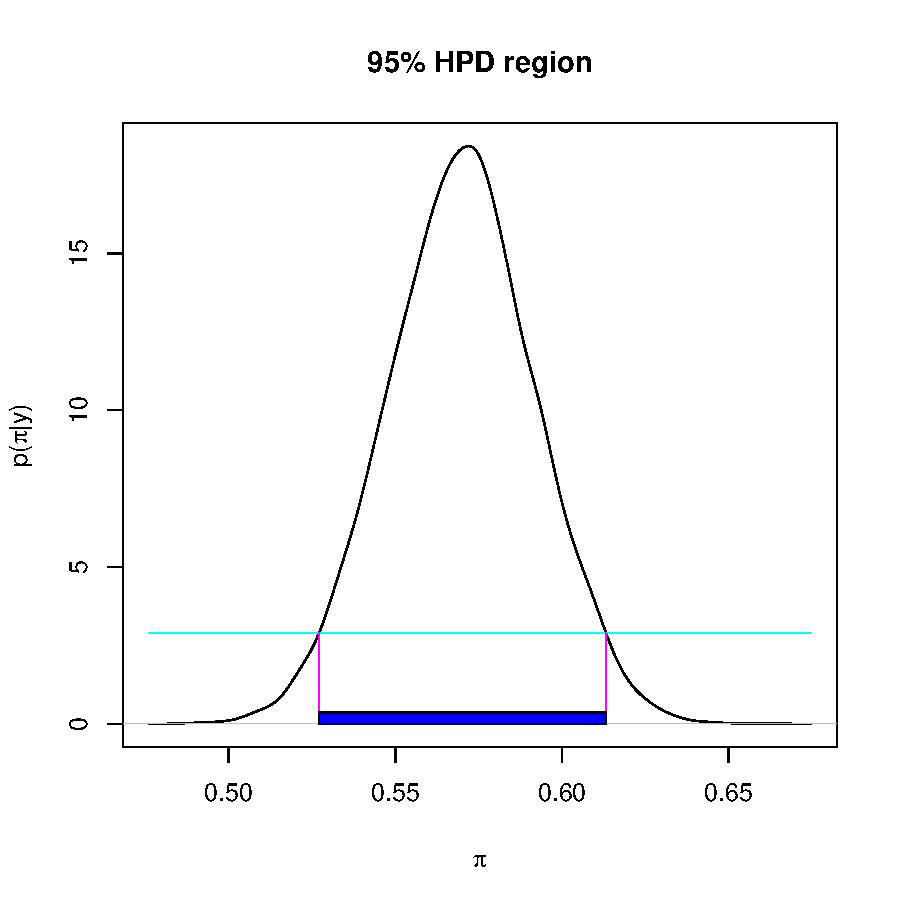
\includegraphics[width = 2in, height = 2in]{summarize-hpd1.pdf}
\end{center}
\end{figure}
\pause
\normalsize
Very similar to central 95\% credible interval for Beta \textcolor{blue}{posterior}.
\end{frame}

\begin{frame}
What about for this \textcolor{blue}{posterior}?
\begin{figure}[!htp]
\begin{center}
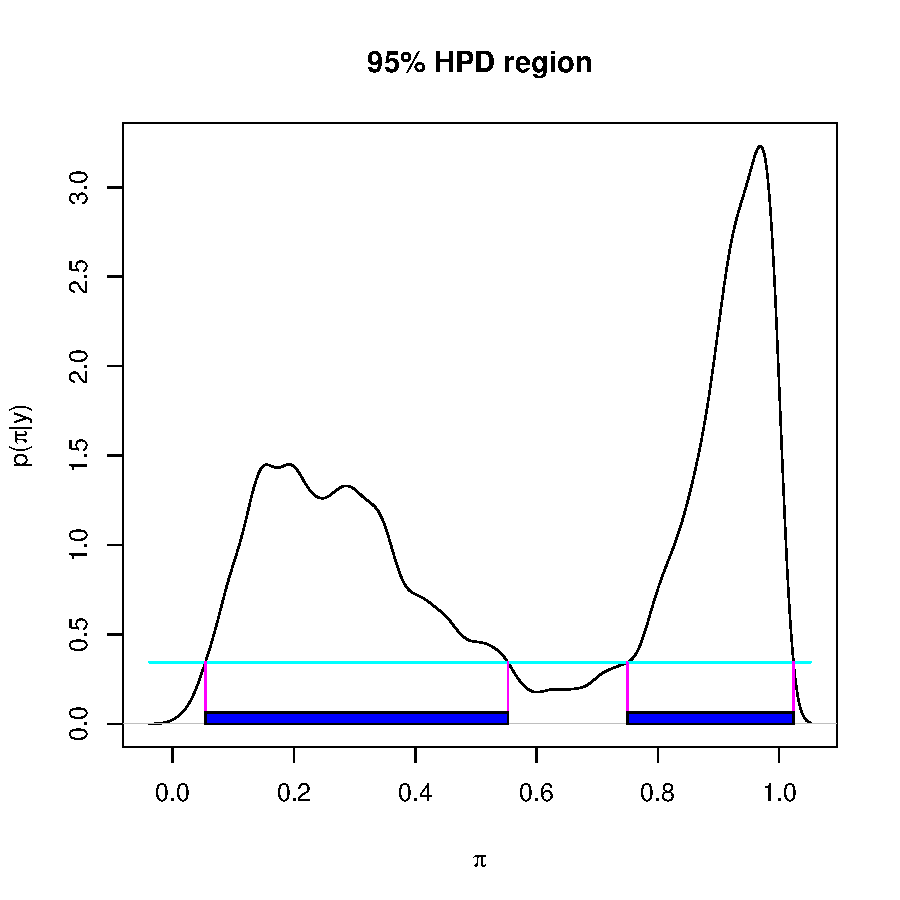
\includegraphics[width = 2in, height = 2in]{summarize-hpd2.pdf}
\end{center}
\end{figure}
\end{frame}

\end{document}
